%!TeX program = xelatex

\documentclass[aspectratio=169]{beamer}
\usepackage[english]{babel}
\usepackage{fontspec}
\usepackage{graphicx}
\usepackage{xcolor}
\usepackage{xltxtra}
\usepackage{hyperref}
\usepackage{multicol}
\usepackage{unicode-math}
\usepackage{changepage}
\usepackage{tcolorbox}
\usepackage{booktabs}
\usepackage{appendixnumberbeamer}

\usetheme{Warsaw}
\setbeamertemplate{navigation symbols}{}
\setbeamertemplate{headline}{}
\setbeamertemplate{bibliography item}[text]

\definecolor{MainRed}{RGB}{175,44,34}     % CMYK 3-95-94-29
\definecolor{DarkRed}{RGB}{127,37,2}      % CMYK 22-91-82-46
\definecolor{AltRed}{RGB}{150,40,14}

\definecolor{GoldLight}{RGB}{200,160,110} % CMYK 18-35-60-10
\definecolor{GoldDark}{RGB}{150,121,82}   % CMYK 18-35-60-40

\definecolor{GrayOne}{RGB}{198,198,198}
\definecolor{GrayTwo}{RGB}{160,160,160}
\definecolor{GrayThr}{RGB}{135,135,135}

\definecolor{NearBlack}{RGB}{31,31,31}

\definecolor{Bejevi}{RGB}{201,188,171}
\definecolor{NearWhite}{RGB}{227,227,227}

\setbeamercolor{structure}{fg=MainRed}
\setbeamercolor{palette primary}{fg=white,bg=DarkRed}
\setbeamercolor{palette secondary}{fg=white,bg=MainRed}
\setbeamercolor{palette tertiary}{fg=white,bg=DarkRed}
\setbeamercolor{palette quaternary}{fg=white,bg=MainRed}

\setbeamercolor{title}{fg=white,bg=MainRed}
\setbeamercolor{frametitle}{fg=white,bg=MainRed}
\setbeamercolor{titlelike}{fg=white,bg=MainRed}

\setbeamercolor{normal text}{fg=black,bg=white}

\setbeamercolor{block title}{fg=white,bg=DarkRed}
\setbeamercolor{block body}{fg=black,bg=DarkRed!8}

\setbeamercolor{block title alerted}{fg=white,bg=MainRed}
\setbeamercolor{block body alerted}{fg=black,bg=MainRed!10}

\setbeamercolor{block title example}{fg=white,bg=GoldDark}
\setbeamercolor{block body example}{fg=black,bg=GoldLight!20}

\setbeamercolor{title in head/foot}{fg=white,bg=DarkRed}
\setbeamercolor{author in head/foot}{fg=white,bg=NearBlack}
\setbeamercolor{date in head/foot}{fg=white,bg=GrayTwo}

\setbeamertemplate{footline}{
        \leavevmode%
        \hbox{%
                \begin{beamercolorbox}[wd=.72\paperwidth,ht=2.8ex,dp=1.2ex,leftskip=1em]{title
                        in head/foot}%
                        \insertshorttitle
                \end{beamercolorbox}%
                \begin{beamercolorbox}[wd=.14\paperwidth,ht=2.8ex,dp=1.2ex,center]{author
                        in head/foot}%
                        Шаго П. Е.
                \end{beamercolorbox}%
                \begin{beamercolorbox}[wd=.14\paperwidth,ht=2.8ex,dp=1.2ex,center]{date
                        in head/foot}%
                        \insertframenumber/\inserttotalframenumber
                \end{beamercolorbox}%
        }%
        \vskip0pt%
}

\tcbuselibrary{skins}
\newtcolorbox{shadowbox}{
        enhanced,
        colback=GrayOne,
        colframe=white,
        boxrule=0pt,
        sharp corners=all,
        arc=6pt,
        drop shadow,
        left=4mm,
        right=4mm,
        top=2mm,
        bottom=2mm
}

\newtcolorbox{shadowbox2}{
        enhanced,
        colback=NearWhite,
        colframe=white,
        boxrule=0pt,
        arc=4pt,
        outer arc=4pt,
        fuzzy shadow={
        0mm}{-1.3mm}{0mm}{0.3mm}{black!30
        },
        coltext=NearBlack,
        halign=center,
        fontupper=\centering,
        left=4mm,
        right=4mm,
        top=2mm,
        bottom=2mm
}

\newtcolorbox{shadowbox3}{
        enhanced,
        colback=NearWhite,
        colframe=MainRed,
        coltext=NearBlack,
        arc=6pt,
        boxrule=0.6pt,
        left=4mm, right=4mm, top=2mm, bottom=2mm,
        halign=center
}

\setmainfont{Iosevka NFM}
\setmonofont{Iosevka NFM}
\setsansfont{Iosevka NFM}
\setromanfont{Iosevka NFM Italic}
\setmathfont{Latin Modern Math}

\title{Математическое моделирование и
        реализация планировщика
процессов для гетерогенных процессорных архитектур}

\begin{document}

\begin{frame}[plain]
        \begin{center}
                \begin{shadowbox3}
                        {\scriptsize
                                Санкт-Петербургский государственный
                                университет \\ [0.1em]
                                Факультет прикладной математики~-- процессов
                                управления \\ [-0.4em]
                                ООП СВ.5005.2022 Прикладная
                                математика, фундаментальная информатика и
                                программирование
                        }
                \end{shadowbox3}
        \end{center}

        \vspace{0.3em}
        {\color{MainRed}\hrule height 1pt}
        \vspace{0.3em}

        \begin{center}
                {\small\color{MainRed}\textbf{Шаго Павел Евгеньевич}}

                \vspace{0.2em}
                \begin{shadowbox3}
                        {\bfseries
                                Математическое моделирование и
                                реализация планировщика
                        процессов для гетерогенных процессорных архитектур}
                \end{shadowbox3}

                \vspace{0.1em}
                {\small\itshape Бакалаврская работа}
        \end{center}
        \vspace{0.5em}

        \begin{minipage}{\textwidth}
                \begin{minipage}[t]{0.45\linewidth}
                        \raggedright
                        {\scriptsize
                                \textit{Научный руководитель:}\\[0.15em]
                                кандидат физ.-мат. наук, доцент\\
                        Корхов В.\,В.}
                \end{minipage}
                \hfill
                \begin{minipage}[t]{0.45\linewidth}
                        \raggedright
                        {\scriptsize
                                \textit{Рецензент:}\\[0.15em]
                                эксперт по архитектуре и сетевому стеку,\\
                        ООО НИЦ АЭРОДИСК, Анохин Ю.\,В.}
                \end{minipage}
        \end{minipage}

        \vfill
        {\color{MainRed}\hrule height 1pt}

        \begin{center}
                {\scriptsize
                        Санкт-Петербург\\[-0.5em]
                2026}
        \end{center}
\end{frame}


\begin{frame}{Постановка задачи}
        \begin{columns}[T]
                \column{0.5\textwidth}
                \begin{itemize}\setlength{\itemsep}{0.3em}
                        \item Современные процессоры все чаще гетерогенны.
                                Объединяют производительные P\nobreakdash-ядра +
                                энергоэффективные E\nobreakdash-ядра

                        \item Linux EEVDF учитывает типы ядер ограниченно,
                                не балансирует производительность и
                                энергопотребление так, как задумано
                                архитектурой CPU
                \end{itemize}

                \column{0.5\textwidth}
                \textbf{Цели работы}
                \begin{enumerate}\setlength{\itemsep}{0.3em}
                        \item Формализовать распределение слотов
                                P/E\nobreakdash-ядер как динамический
                                аукцион Викри (VCG)

                        \item Реализовать механизм используя \texttt{sched\_ext}
                                и оценить на тестах производительности
                \end{enumerate}
        \end{columns}

        \vspace{0.3em}
        \begin{shadowbox2}
                \small Каждое ядро рассматривается как
                \textbf{истощаемое благо}, неиспользованный квант
                времени теряется безвозвратно. Задача\nobreakdash-агент
                характеризуется типом $\theta_i = (v_i, l_i)$, а
                механизм максимизирует социальное благосостояние.
        \end{shadowbox2}
\end{frame}


\begin{frame}{Модель системы}
        \begin{columns}[T]
                \column{0.5\textwidth}
                \textbf{Аппаратная платформа}
                \begin{itemize}
                        \item Ядра: $\mathcal{P} = \{P_1,\ldots,P_{K_P}\}$,\;
                                $\mathcal{E} = \{E_1,\ldots,E_{K_E}\}$
                        \item Дискретное время $t = 1,2,3,\ldots$
                        \item Замедление на E-ядре:
                                $\sigma = \eta_P/\eta_E > 1$
                        \item Общий ISA (любая задача может быть
                                выполнена на любом ядре)
                \end{itemize}

                \column{0.5\textwidth}
                \textbf{Задачи как агенты}
                \begin{itemize}
                        \item Тип $\theta_i = (v_i, l_i)$ (оценка и длина)
                        \item Полезность $u_i = v_i - p_i$ при полном
                                выполнении
                        \item Бюджет $B_i$ по классу обслуживания:
                \end{itemize}
                \vspace{0.2em}
                {\footnotesize
                        \begin{tabular}{@{}ll@{}}
                                Реального времени & $B_{RT} \gg 1$ \\
                                Интерактивный     & $B_{int}$ \\
                                Пакетный          & $B_{batch}$ \\
                                Фоновый           & $B_{bg} \approx 0$
                \end{tabular}}
        \end{columns}

        \vspace{0.4em}
        \begin{shadowbox}
                \footnotesize На E-ядре задача длиной $l_i$ исполняется за
                $\lceil l_i \cdot \sigma \rceil$ квантов.
                Ценность $v_i$ начисляется только при полном выполнении
                (условие полного исполнения по Sano, 2023).
        \end{shadowbox}
\end{frame}


\begin{frame}{MDP модель}
        \begin{columns}[T]
                \column{0.5\textwidth}
                \textbf{Состояние} $s^t =
                (\mathbf{x}^t,\,\mathbf{b}^t,\,\boldsymbol{\omega}^t)$
                \begin{itemize}
                        \item $\mathbf{x}^t$~-- оставшиеся кванты на
                                каждом ядре
                        \item $\mathbf{b}^t$~-- остатки бюджетов активных задач
                        \item $\boldsymbol{\omega}^t$~-- внешние факторы
                                (температура, нагрузка)
                \end{itemize}

                \vspace{0.3em}
                \textbf{Действие}  $a^t = (a_{i,P}^t, a_{i,E}^t)_i$
                при ограничениях:
                $$a_{i,P}^t + a_{i,E}^t \leq 1, \quad \forall i$$
                $$\sum_i a_{i,P}^t \leq K_P^t, \quad
                \sum_i a_{i,E}^t \leq K_E^t$$

                \column{0.5\textwidth}
                \textbf{Вознаграждение}

                \vspace{0.2em}
                Задача $i$ (покупатель):
                $$r_i(s,a) = v_i \cdot \mathbb{1}[\text{$i$ завершилась в $t$}]$$

                Планировщик (продавец):
                $$r_0 = \mu_P\!\!\sum_{k\in\mathcal{P}}\!\mathbb{1}[x_k \geq 1]
                + \mu_E\!\!\sum_{k\in\mathcal{E}}\!\mathbb{1}[x_k \geq 1]$$

                \vspace{0.1em}
                {\footnotesize $\mu_\kappa$~-- вознаграждение за активный
                квант ядра типа~$\kappa$;\, $\mu_P > \mu_E$
                (P\nobreakdash-ядро производительнее)}

                \vspace{0.2em}
                \textbf{Социальное благосостояние}
                $$W(\pi) = \lim_{T\to\infty} \frac{1}{T}
                \mathbb{E}\!\left[\sum_{t=1}^T R(s^t,a^t)\right]$$
        \end{columns}
\end{frame}


\begin{frame}{Механизм VCG}
        \textbf{Эффективная ценность} задачи $i$ на ядре типа
        $\kappa \in \{P, E\}$
        $$\phi_P(\theta_i) = v_i - c_P \cdot l_i, \quad
        \phi_E(\theta_i) = v_i - c_E \cdot \lceil l_i \sigma \rceil$$

        \vspace{0.1em}
        \textbf{Оптимальное распределение} (максимизация $W$)
        $$a^t = \arg\max_{a} \sum_i \bigl[a_{i,P}\,\phi_P(\theta_i)
        + a_{i,E}\,\phi_E(\theta_i)\bigr]
        + \delta\, \mathbb{E}[W(s^{t+1})]$$
        {\footnotesize $\delta \in [0,1)$~-- дисконт будущего благосостояния}

        \vspace{0.1em}
        \begin{columns}[T]
                \column{0.52\textwidth}
                \textbf{Платёж VCG} задачи $i$
                $$p_i^t = W_{-i}(s^t) - \bigl(W(s^t) -
                \phi_\kappa(\theta_i)\bigr)$$

                \vspace{0.1em}
                {\footnotesize $W(s^t),\,W_{-i}(s^t)$~-- оптимальное
                социальное благосостояние с~$i$ и без неё. Задача $i$
                платит ровно то, что теряют остальные агенты из-за её
                присутствия (pivot rule).}

                \column{0.48\textwidth}
                \begin{shadowbox}
                        \footnotesize
                        \textbf{Свойства механизма}
                        \centering
                        \begin{itemize}
                                \item Стимульная совместимость
                                        (в~пределах класса, см.~Extra)
                                \item Индивидуальная рациональность
                                        $u_i \geq 0$
                                \item Бюджетное ограничение
                                        $p_i \leq B_i^t$
                        \end{itemize}
                \end{shadowbox}
        \end{columns}
\end{frame}


\begin{frame}{Маршрутизация задач}
        \textbf{Сигнал маршрутизации}~-- отношение бюджета
        $\rho_i = B_i / B_i^{\max}$
        {\footnotesize (высокое $\rho$ $\Leftrightarrow$ много накопленного
        бюджета $\Leftrightarrow$ недавний простой)}

        \vspace{0.3em}
        \begin{columns}[T]
                \column{0.33\textwidth}
                \begin{shadowbox2}
                        \small\textbf{DSQ\_P}

                        \vspace{0.3em}
                        \footnotesize
                        $\rho_i \geq \rho^*\ (50\%)$

                        \vspace{0.2em}
                        Задача короткими всплесками
                        потребляет CPU и большую
                        часть времени ждёт IO.
                        Выигрывает от пиковой
                        частоты P-ядра
                \end{shadowbox2}

                \column{0.33\textwidth}
                \begin{shadowbox2}
                        \small\textbf{DSQ\_E}

                        \vspace{0.3em}
                        \footnotesize
                        $\rho_i < \rho^*$

                        \vspace{0.2em}
                        Задача устойчиво расходует
                        бюджет, близка к CPU-bound

                        переносима на E-ядро
                \end{shadowbox2}

                \column{0.33\textwidth}
                \begin{shadowbox2}
                        \small\textbf{DSQ\_Starved}

                        \vspace{0.3em}
                        \footnotesize
                        $B_i < B_i^{\max} / 10$

                        \vspace{0.2em}
                        Бюджет почти исчерпан
                        штраф к виртуальному
                        дедлайну
                        $v_d \mathrel{+}=
                        \max(0,\,-\phi_\kappa)\,/\,D$

                        \vspace{0.1em}
                        {\scriptsize демоция,
                        не блокирует остальных}
                \end{shadowbox2}
        \end{columns}

        \vspace{0.3em}
        \begin{shadowbox}
                \footnotesize Прирост бюджета за время простоя
                $B_i \mathrel{+}= \Delta t_{\text{idle}} \cdot v_i
                / D_{\text{rep}}$ играет роль, аналогичную пороговому
                правилу Майерсона в одномерных аукционах
        \end{shadowbox}
\end{frame}


\begin{frame}{sched\_ext}
        \begin{shadowbox2}
                \small \textbf{sched\_ext} (scheduler extensions)~--
                инфраструктура ядра Linux, позволяющая реализовывать
                политику планирования как eBPF-программу,
                подключаемую к хукам планировщика без пересборки ядра
        \end{shadowbox2}

        \vspace{0.3em}
        \begin{columns}[T]
                \column{0.50\textwidth}
                % TODO(tasks/scx_diagram.md): заменить на схему sched_ext
                % (DSQ, цикл select_cpu/enqueue/dispatch). Текущая
                % картинка иллюстрирует eBPF на сетевом стеке.
                \vspace{0.3em}
                \centering
                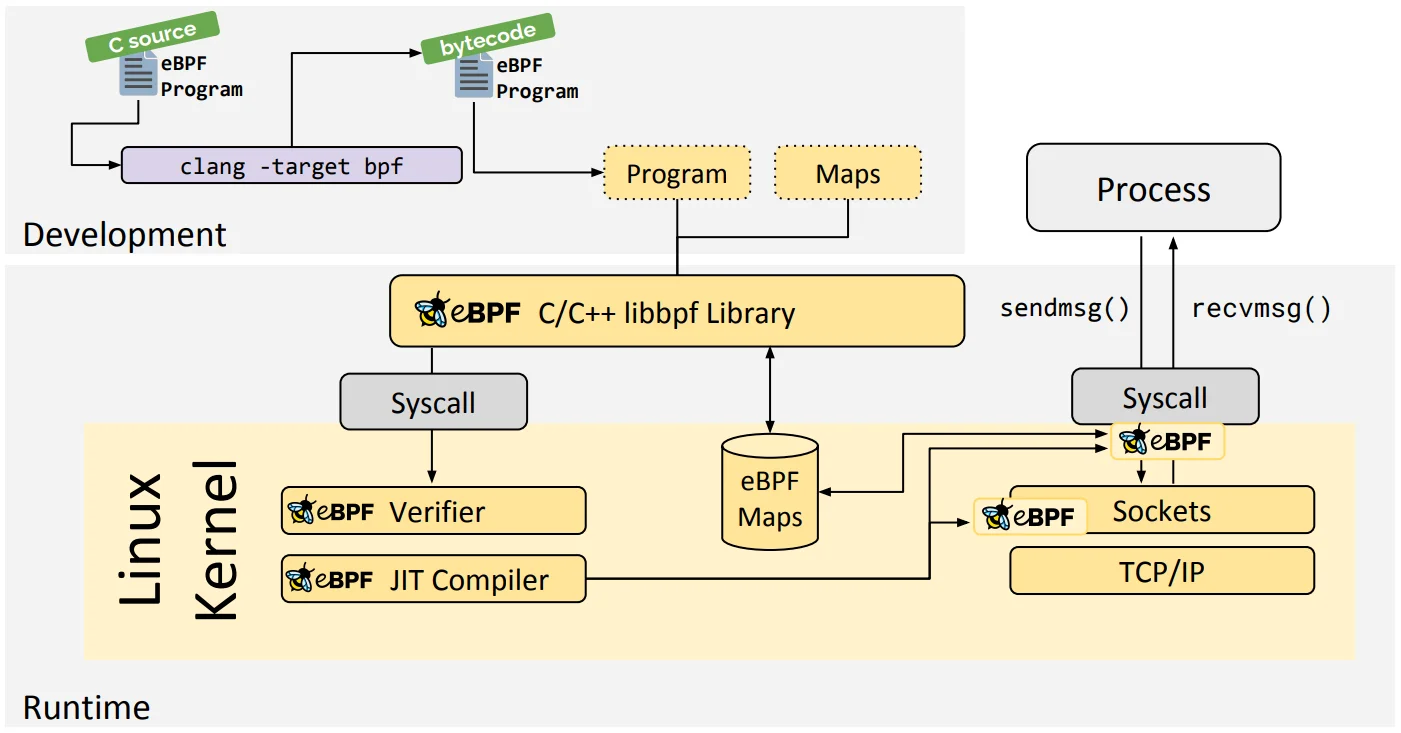
\includegraphics[width=\linewidth]{../0212/res/libbpf.png}

                \vspace{0.1em}
                {\tiny \textbf{Рис.~1.} eBPF как общая инфраструктура
                ядра Linux}

                \column{0.50\textwidth}
                \textbf{DSQ} (dispatch queue):
                {\footnotesize
                        \begin{itemize}
                                \item \texttt{SCX\_DSQ\_LOCAL}~--
                                        локальная очередь ядра
                                \item \texttt{SCX\_DSQ\_GLOBAL}~--
                                        общая очередь
                                \item пользовательские DSQ по любому критерию
                \end{itemize}}

                \vspace{0.2em}
                \textbf{Цикл планирования}
                {\footnotesize
                        \begin{itemize}
                                \item \texttt{select\_cpu}~-- выбор
                                        свободного ядра
                                \item \texttt{enqueue}~-- помещение
                                        задачи в DSQ
                                \item \texttt{dispatch}~-- перенос в
                                        локальный DSQ
                                \item \texttt{running} / \texttt{stopping}~--
                                        обновление vtime
                \end{itemize}}
        \end{columns}
\end{frame}


\begin{frame}{Среда тестирования}
        \begin{columns}[T]
                \column{0.24\textwidth}
                \begin{shadowbox}
                        \small\textbf{Система}

                        \vspace{0.25em}
                        \footnotesize
                        Ядро Linux 7.0

                        \vspace{0.25em}
                        CPU: Intel Core\\ Ultra 7 265K\\
                        8P + 12E
                \end{shadowbox}

                \begin{shadowbox}
                        \small\textbf{Сравнение}

                        \vspace{0.2em}
                        \footnotesize
                        Linux EEVDF\\
                        \textit{vs}\\
                        scx\_EEVDF\\
                        \textit{vs}\\
                        scx\_LAVD\\
                        \textit{vs}\\
                        scx\_auction (VCG)
                \end{shadowbox}

                \column{0.52\textwidth}
                \begin{shadowbox}
                        \small\textbf{Бенчмарки}

                        \vspace{0.15cm}
                        \footnotesize
                \begin{itemize}\setlength{\itemsep}{0.15cm}\setlength{\parskip}{0pt}
                                \item \textbf{hackbench}~-- 10 групп по 40
                                        задач, обмениваются короткими
                                        сообщениями через сокеты.
                                        Генерирует большое количество
                                        переключений контекста (стресс тест
                                        для планировщиков)

                                \item \textbf{sysbench}~-- нагрузка на CPU,
                                        память и дисковый ввод-вывод
                                        с параметрами по умолчанию.
                                        Имитирует смешанную OLTP-нагрузку
                                        баз данных

                                \item \textbf{sched\_latency}~-- собственный
                                        тест, работает параллельно с нагрузкой.
                                        Регистрирует, сколько задача ждёт
                                        между моментом готовности и
                                        началом исполнения
                        \end{itemize}
                \end{shadowbox}

                \column{0.24\textwidth}
                \begin{shadowbox}
                        \small\textbf{Метрики}

                        \vspace{0.15cm}
                        \footnotesize
                        \textbf{hackbench}\\
                        Время ($s$), $\downarrow$

                        \vspace{0.15cm}
                        \textbf{sysbench}\\
                        events$/s$, $\uparrow$

                        \vspace{0.15cm}
                        \textbf{sched\_latency}\\
                        p99 ($\mu s$) по типам

                        \vspace{0.15cm}
                        \textbf{RAPL}\\
                        package ($W$)
                \end{shadowbox}

        \end{columns}
\end{frame}


\begin{frame}{Результаты. Hackbench}
        \begin{center}
                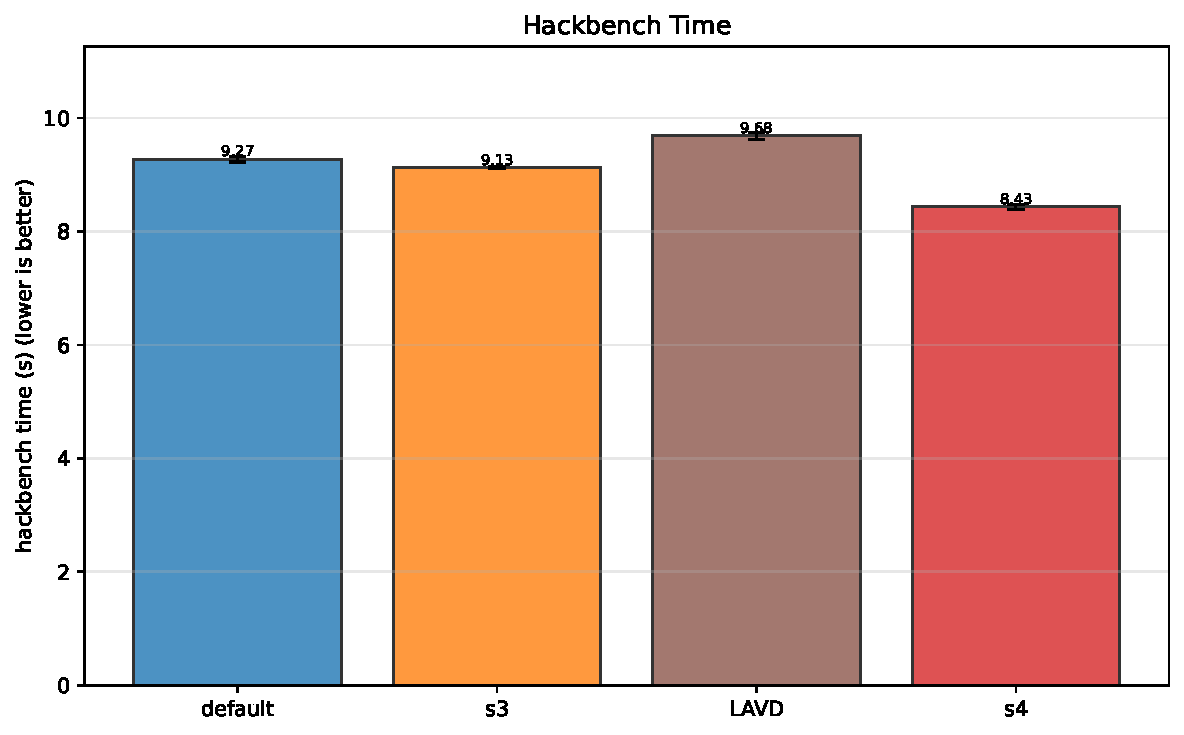
\includegraphics[width=0.86\linewidth]{res/throughput_hackbench.pdf}
        \end{center}
\end{frame}


\begin{frame}{Результаты. Sysbench}
        \begin{center}
                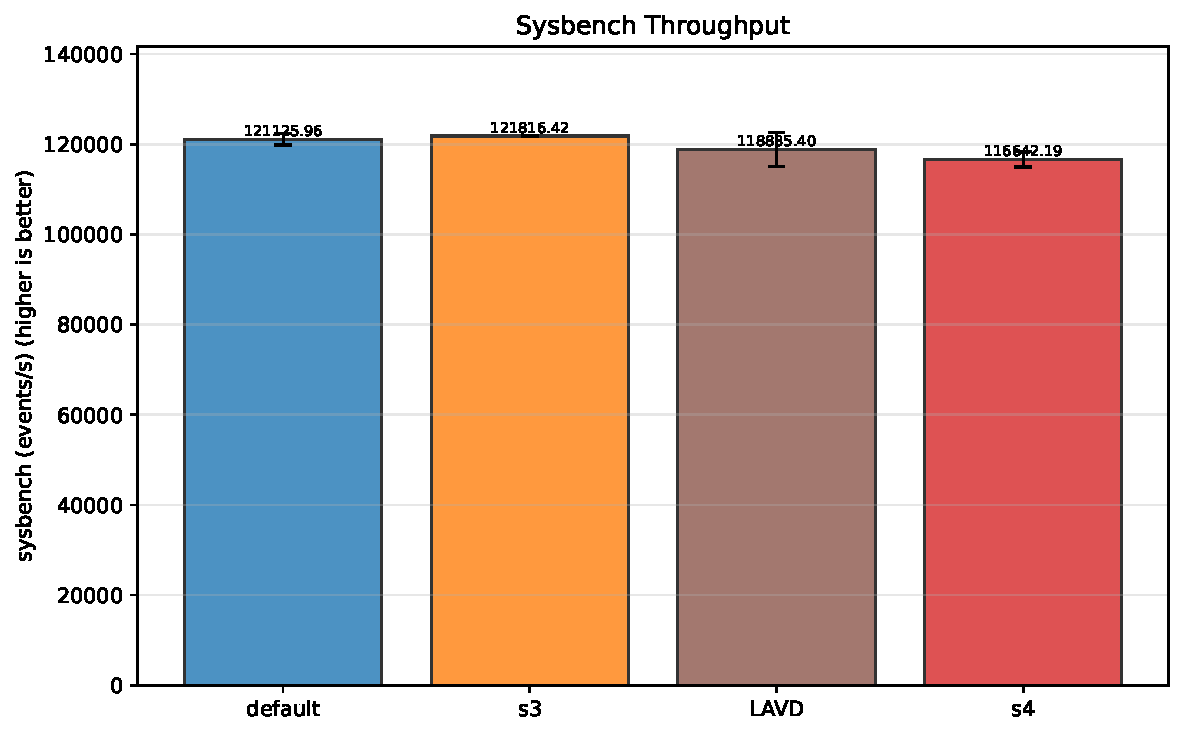
\includegraphics[width=0.86\linewidth]{res/throughput_sysbench.pdf}
        \end{center}
\end{frame}


\begin{frame}{Результаты. Итоговая таблица}
        \vspace{0.3em}
        \begin{center}
                {\small
                        \begin{tabular}{@{}lrrrr@{}}
                                \toprule
                                \textbf{Метрика} & \textbf{Linux
                                EEVDF} & \textbf{scx\_EEVDF} &
                                \textbf{scx\_LAVD} & \textbf{scx\_auction} \\
                                \midrule
                                Hackbench (s)~$\downarrow$         &
                                9.27 & 9.13 & 9.68 & \textbf{8.43} \\
                                Sysbench (ev/s)~$\uparrow$         &
                                121\,126 & \textbf{121\,816} &
                                118\,835 & 116\,642 \\
                                Sched delay avg ($\mu$s)~$\downarrow$
                                & 2172 & 4620 & \textbf{361} & 3629 \\
                                Sched delay p99 ($\mu$s)~$\downarrow$
                                & 9605 & 15\,246 & \textbf{3014} & 38\,025 \\
                                Preemption avg ($\mu$s)~$\downarrow$
                                & 8878 & \textbf{18} & 9709 & 1055 \\
                                Context sw (K/s)~$\downarrow$      &
                                187 & \textbf{46} & 191 & 62 \\
                                Sleep dur. avg (ms)~$\downarrow$   &
                                130 & 149 & 113 & \textbf{26} \\
                                Power (W)~$\downarrow$             &
                                175.7 & 187.8 & \textbf{167.4} & 186.5 \\
                                \bottomrule
                        \end{tabular}
                }
        \end{center}
\end{frame}


\begin{frame}{Список литературы \& Вопросы}
        \begin{thebibliography}{20}
                \scriptsize

                \bibitem{leon}
                Leon~G., Etesami~O.
                Mechanism Design for Scheduling with Heterogeneous Workers.
                NeurIPS, 2022

                \bibitem{sano}
                Sano~T.
                Dynamic Mechanism Design for Multi-Period Contracting.
                Working paper, 2023

                \bibitem{myerson}
                Myerson~R.~B.
                Optimal Auction Design.
                Mathematics of Operations Research, 6(1), 1981, pp.~58--73

                \bibitem{stoica}
                Stoica~I., Abdel-Wahab~H.
                Earliest Eligible Virtual Deadline First: A Flexible and
                Accurate Mechanism for Proportional Share Resource Allocation.
                Old Dominion University, 1996

                \bibitem{schedext_arxiv}
                Agrawal~A., Banerjee~S., Barford~P. et~al.
                sched\_ext: A BPF-extensible Linux Scheduler.
                arXiv:2408.01997, 2024

                \bibitem{ghost}
                Humphries~J.\,T., Natu~N., Chaugule~A. et~al.
                ghOSt: Fast \& Flexible User-Space Delegation of
                Linux Scheduling.
                ACM SOSP, 2021

                \bibitem{pie}
                Van~Craeynest~K., Jaleel~A., Eeckhout~L. et~al.
                Scheduling Heterogeneous Multi-Cores through
                Performance Impact Estimation (PIE).
                ISCA, 2012, pp.~213--224

                \bibitem{galin}
                Galin~M., Hedblom~A.
                Linux Kernel Scheduler Evaluation for Performance-Critical
                Telecom Workloads.
                Linköping University, 2025

                \bibitem{sched_ext}
                \href{https://lwn.net/Articles/922405}
                {The extensible scheduler class (LWN)}

                \bibitem{eevdf}
                \href{https://lwn.net/Articles/925371}
                {An EEVDF CPU scheduler for Linux (LWN)}

        \end{thebibliography}
\end{frame}


\appendix

\begin{frame}{Extra}
        \textbf{Стимульная совместимость (Sano, Теорема~1)}

        \vspace{0.2cm}
        Механизм стимульно совместим тогда и только тогда, когда
        для каждой задачи $i$:

        \begin{enumerate}
                \item $\alpha_i(v_i, l_i)$ не убывает по $v_i$
                        при фиксированном $l_i$
                \item $\int_0^{v_i} \alpha_i(\nu, l_i)\,d\nu$ не возрастает
                        по $l_i$ при фиксированном $v_i$
                \item Существует $\underline{\Pi}_i$, не зависящее от $l_i$:
                        $$\Pi_i(v_i, l_i) = \underline{\Pi}_i +
                        \int_0^{v_i} \alpha_i(\nu, l_i)\,d\nu$$
        \end{enumerate}

        \vspace{0.1cm}
        \begin{shadowbox}
                \footnotesize Задачам невыгодно завышать оценку $v_i$
                или занижать длину $l_i$~--- правдивая ставка
                является доминирующей стратегией
        \end{shadowbox}
\end{frame}
\addtocounter{framenumber}{-1}

\begin{frame}{Extra}
        \textbf{Онлайн-обучение: IHMDP-VCG (Leon \& Etesami)}

        \vspace{0.15cm}
        При неизвестных распределениях типов задач и ядре MDP планировщик
        обучается онлайн. Эпизодическая структура:

        \begin{itemize}
                \item \textbf{Фаза перемешивания} (длина $d^{[k]}$):
                        вывод цепи Маркова на стационарное распределение
                \item \textbf{Стационарная фаза} (длина $l^{[k]}$):
                        сбор платежей $\hat{p}^{[k]}$, обновление оценок
        \end{itemize}

        \vspace{0.15cm}
        \textbf{Гарантии} при $T \to \infty$ (с вер. $\geq 1 - O(\zeta)$):

        \vspace{0.1cm}
        \begin{columns}
                \column{0.5\textwidth}
                \begin{tabular}{ll}
                        Регрет благосостояния &
                        $\tilde{O}(\varepsilon T n + T^{2/3} n)$ \\[3pt]
                        Регрет продавца &
                        $\tilde{O}(\varepsilon T n^2 + T^{2/3} n^2)$ \\[3pt]
                        Регрет покупателей &
                        $\tilde{O}(\varepsilon T n^2 + T^{2/3} n^2)$
                \end{tabular}

                \column{0.5\textwidth}
                \begin{shadowbox}
                        \footnotesize Асимптотически: эффективность,
                        стимульная совместимость и индивидуальная
                        рациональность~--- одновременно
                \end{shadowbox}
        \end{columns}
\end{frame}
\addtocounter{framenumber}{-1}

\begin{frame}{Extra}
        \textbf{Пример: $K_P = K_E = 1$, одно свободное ядро типа $\kappa$}

        \vspace{0.2cm}
        \textbf{Победитель:}
        $$i^* = \arg\max_{i \in \mathcal{N}^t,\; B_i^t > 0}\;
        \phi_\kappa(\theta_i) + \delta^{m_\kappa(l_i)}\,\bar{W}_\kappa$$

        где $m_P(l) = l$,\; $m_E(l) = \lceil l\cdot\sigma \rceil$

        \vspace{0.2cm}
        \textbf{Платёж победителя:}
        $$p_{i^*} = \phi_\kappa^{-1}\!\left(\phi_\kappa(\theta_j) +
                \bigl(\delta^{m_\kappa(l_j)} - \delta^{m_\kappa(l_{i^*})}\bigr)
        \bar{W}_\kappa \;\Big|\; l_{i^*}\right)$$

        где $j$~--- задача на втором месте.

        \vspace{0.2cm}
        \begin{shadowbox}
                \footnotesize
                $\phi_P(\theta_i) > \phi_E(\theta_i)$ выполняется не всегда:
                при малом $v_i$ и большом $l_i$ E-ядро может дать
                большую эффективную ценность ($c_E \cdot \lceil l_i\sigma\rceil
                < c_P \cdot l_i$ при $\sigma < \gamma$).
                Оптимальная стратегия нетривиальна.
        \end{shadowbox}
\end{frame}
\addtocounter{framenumber}{-1}

\begin{frame}{Extra}
        \textbf{IC при жёстком бюджетном ограничении}

        \vspace{0.15cm}
        \textbf{Проблема.} В классическом VCG
        $p_i^{\text{VCG}} > B_i$ создаёт стимул к~искажению ставки,
        чтобы попасть в~допустимое множество~--- IC ломается
        \footnotesize{(Dobzinski, Lavi, Nisan 2008)}.

        \vspace{0.15cm}
        \textbf{Наш случай.} Бюджет $B_i$~--- функция класса обслуживания
        $\kappa_i\in\{\text{RT},\text{int},\text{batch},\text{bg}\}$,
        фиксированного приоритетом процесса
        (\texttt{policy}/\texttt{nice}) до поступления в~механизм.
        Класс~--- public type, не~объект стратегии.

        \vspace{0.15cm}
        \begin{shadowbox}
                \footnotesize
                \textbf{Утверждение.} При фиксированном классе $\kappa$
                и~соответствующем бюджете $B(\kappa)$ механизм
                IC на~подтипе $(v_i, l_i)$: условия Sano (Т.~1)
                выполняются для $\alpha_i^\kappa$, платёж
                $p_i \leq B(\kappa)$ не~зависит от сообщения
                агента~$\Rightarrow$ правдивое $(v_i, l_i)$~---
                доминирующая стратегия внутри класса.
        \end{shadowbox}

        \vspace{0.1cm}
        {\scriptsize Между классами~--- approximate IC; задача с~$p_i^{\text{VCG}} > B_i$
        отсекается аллокацией (§8.3 модели), не~перепрайсингом.}
\end{frame}
\addtocounter{framenumber}{-1}

\end{document}
